\chapter{Introduction}

\section{Context}

\par
%Identify the problem
Programming is like building something with primitive blocks and it can be a very difficult task if we have to program every aspect of the application without some “blocks” already built for us to use.
That’s why in the programming world there is a whole panoply of free and commercial libraries with APIs that provide a huge quantity of functions for the programmer to use.

\par
In computer graphics, there are many 3D graphics libraries that provide functionalities to render images based in different techniques.
Two of the most used render techniques are rasterization and ray tracing.
Ray tracing can be used to calculate and simulate the path of particles and waves.
It can simulate the propagation of sound, the path of light and even allows to simulate technologies developed by men like the Wi-fi networks.
It can render an image by tracing the path of light through pixels in an image plane and simulating the effects of its interactions with virtual objects.
It can render much more realistic shadows, reflections and refractions and in an easier way than rasterization.
This technique is capable of producing a very high degree of visual realism but at a great computational cost.

\par
Since nowadays we have more and more mobile systems whose computational power increases every year, the need for more libraries to help the programmers develop applications for these systems is increasing too.
However, there are not many options to choose from for developing a renderer based on ray tracing.
That’s why this dissertation focuses on assessing and providing a ray tracer library for mobile systems.

\par
%To delimit the problem
It is important to mention that this dissertation is not focused on rendering techniques other than ray tracing.
It is not focused in assess different integrators (numerical solutions to the rendering equation) and / or assess different approaches in ray tracing like Packet Traversal.
It is also not focused on assess different quasi random numbers generators neither assess the performance of different computer systems.

\par
These rendering algorithms based in ray tracing are very useful because they allow rendering photo-realistic images with a degree of realism much better than the graphics cards allow by default through rasterization.
As previously stated, the computing power in mobile devices processors has been increasing and this may allow a mobile device with a mid-range processor to run these algorithms in a useful time.

\begin{figure}[H]
\centering
\caption{Illustration of the most common mobile devices - tablet and smartphone (\cite{JournalDuNet}).}
\label{Illustration of the most common mobile devices - tablet and smartphone}
\includegraphics[width=10cm,height=10cm,keepaspectratio,scale=1.0]{Mobile_devices.jpg}
\end{figure}

\section{Motivation}

\par
Among other factors, the productivity of a programmer depends on what libraries he can have access to.
But, there are almost no rendering libraries based in ray tracing available today for mobile systems like Android, iOS, Windows 10 Mobile, BlackBerry 10, Tizen, Sailfish OS, Symbian and Ubuntu Touch.
And it is likely that these systems already have enough processing power to render images with fairly complex scenes in an acceptable time by using algorithms based in ray tracing.

\par
It is also important to note that there is not much documentation about the advantages and limitations of executing different rendering algorithms in these devices.

\par
Last but not least, it is important to mention that of all the operating systems available for mobile devices, the one chosen for this ray tracing library was Android.
Because nowadays it is the operating system with the most market share.
More than 85\% of the mobile devices use Android, and only 14\% of these devices use iOS which is the second most used operating system in these devices.
And, besides that, it allows to be executed on a variety of different devices: smart phones, tablet computers, smart TVs, smart watches and even laptop / desktop computers.

\begin{figure}[H]
	\centering
	\caption{Illustration of a variety of mobile devices compatible with Android (\cite{AndroidDevices}).}
	\label{Illustration of a variety of mobile devices compatible with Android}
	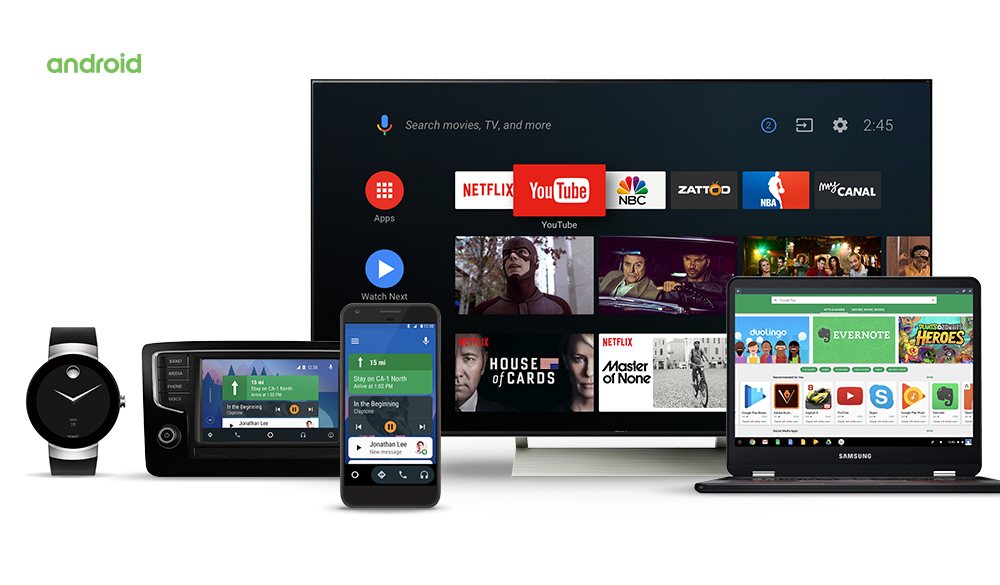
\includegraphics[width=10cm,height=10cm,keepaspectratio,scale=1.0]{Android_devices.png}
\end{figure}


\section{Goals}

\par
The main goal of this dissertation is to assess and demonstrate the advantages of running rendering algorithms in mobile devices.

\par
It is also intended to promote and facilitate the development of applications for mobile systems that use ray tracing techniques, with special emphasis on rendering applications.
To do this, it will be developed a library that supports the fundamental operations of a ray tracing engine.
This library will allow the agile development of diverse applications, by using components that invoke the functionality of the library itself.

\par
Additionally, it is intended to supply rendering components at a higher abstraction level, like the camera, scene and the integrator that facilitates further the development of applications.

\par
Finally, it is important to do a demonstration of the rendering application with some interface layer to let the user assess the performance of several functionalities provided by the library.

\section{Applications of Ray Tracing}

\par
The subject of this dissertation is about ray tracing because it is a technology widely used in several areas of Computer Graphics.

\par
Ray tracing is a rendering technique that is widely used in the areas of theater and television lighting.
It allows set and lighting designers, actors, and directors to develop and visualize complex lighting setups months before a production ever opens.

\par
Ray tracing is capable of considering all of the light in a given environment which is called Global Illumination.
Global illumination is a physically correct model, which accurately simulates light's behavior in a real physical environment.
Global illumination is a valuable engineering tool in that it allows us to quantitatively analyze the distribution and directionality of light and research radiant heat transfer.

\par
Finally, ray tracing can also be used in the Animation market.
It can be used to add "fancy" effects such as reflection and shadowing that are often difficult and time consuming for traditional artists to produce.
Graphical technology is also capable of rendering photo-realistic images that would be nearly impossible to produce without computerized ray tracing.


\section{Document Structure}

\par
This dissertation is organized in six chapters: Introduction, State of the Art, Software Architecture, Android challenges, Demonstration: Global Illumination and Conclusion \& Future work.

\par
The first chapter describes the context and motivation behind this work, as well as its goals.
Its main purpose is to identify the problem at hand and set up goals that should be accomplished.

\par
The second chapter introduces the main concepts of ray tracing and compares different implementations of ray tracers already available in the world wide web.
The reason behind this comparison is to show how many ray tracers are already available to mobile devices and highlight the differences between the features they provide.
It also provides some information about the processors of today that helps realize their ability to execute computationally demanding algorithms like ray tracing.

\par
The third chapter explains the proposed approach and explains each module developed in the library, as well as each of the rendering components.

\par
The fourth chapter starts with an explanation of some Android specifics, such as the user interface by characterizing its work flow and mentioning some of the benefits and challenges overcame during the development of the application.
It also describes some programming decisions made during the development of the ray tracing library.

\par
The fifth chapter summarizes the key results obtained by executing different algorithms with different number of threads and different acceleration structures.
And concludes with a small comparison of the features provided in this library and an Android ray tracing engine developed by third parties called Android CPU Raytracer (\cite{Android_CPU_Raytracer}).

\par
Finally, the last chapter ends this dissertation with the conclusions that can be withdrawn from this work and proposes some future work.

\par
Last but not least, the Appendix contains this library's API and an example code of how to load a scene from a wavefront obj file.